\section{Temporal cross-phase and generated directional imbalance}\label{sec:timing}
The common-envelope obstruction suggests a general question before selecting any lag: which temporal relationship between two source histories creates an imbalance? The answer combines their finite-time cross-phase with the actual contact angle.~\cite{SRG08} Throughout this section preparation is zero and the mean is retained.

\subsection{General finite-history theorem}
Let real $f_\pm$ have support in $[0,\tf]$ and belong to $L^2$ there; continuous or piecewise continuous histories suffice. Put $\omega_n=nc/R$ and
\begin{equation}\label{eq:finiteF}
 \F_j(\omega)=\int_0^{\tf}f_j(u)e^{+\ii\omega u}\dd u,\qquad
 \F_j^t(\omega)=\int_0^{\min(t,\tf)}f_j(u)e^{+\ii\omega u}\dd u,
 \qquad\beta_n=B_n/L.
\end{equation}
The value at zero is the actual integral. Use one common reference $\tref\ge\tf$ for post-source amplitudes, with the convention
\begin{equation}\label{eq:generalexpansion}
 \begin{aligned}
 p&=\bar p+\sum_{n\ge1}\Re\{(a_{+,n}e^{-\ii n\chi}+a_{-,n}e^{\ii n\chi})e^{\ii\omega_n(t-\tref)}\},\\
 r&=\bar r+\sum_{n\ge1}\Re\{(a_{+,n}e^{-\ii n\chi}-a_{-,n}e^{\ii n\chi})e^{\ii\omega_n(t-\tref)}\}.
 \end{aligned}
\end{equation}

\begin{theorem}[Temporal cross-phase criterion]\label{thm:temporal}
Under these assumptions,
\begin{equation}\label{eq:generalamp}
 a_{\sigma,n}=\beta_ne^{\ii\omega_n\tref}
 \sum_{j=\pm}e^{\sigma\ii ns_j/R}\overline{\F_j(\omega_n)},\qquad
 \bar p=\frac{\F_+(0)+\F_-(0)}L,\quad\bar r=0.
\end{equation}
For each positive $n$, the squared-amplitude difference is
\begin{equation}\label{eq:criterion}
 \boxed{D_n=|a_{+,n}|^2-|a_{-,n}|^2
 =-4\beta_n^2\sin(2n\theta)\Im(\F_+\overline{\F_-})
 =8\beta_n^2\sin(2n\theta)\Im(\F_s\overline{\F_a}).}
\end{equation}
The same identities with truncated transforms hold at each finite time. Furthermore,
\begin{equation}\label{eq:generalaccount}
 E=\frac L2\bar p^2+\sum_{n\ge1}\frac L2(|a_{+,n}|^2+|a_{-,n}|^2),\qquad
 \Jflux=\frac{cL}2\sum_{n\ge1}D_n.
\end{equation}
The series converge; a nonzero term $D_n$ need not imply a nonzero signed sum.
\end{theorem}
\begin{proof}
Multiply \eqref{eq:characteristics} by $\sqrt2$. The unnormalized variable $p+\sigma r$ equals the sum over ports of $\int b_j(s-\sigma c(t-u))f_j(u)\dd u$. Its spatial Fourier coefficient is
$\beta_n\sum_j e^{-\ii ns_j/R}e^{-\sigma\ii\omega_nt}\F_j(\sigma\omega_n)$.
For real inputs $\F_j(-\omega)=\overline{\F_j(\omega)}$. In $p$, recombination contributes $1/2$, whereas expressing a real harmonic as a real part contributes a factor 2. They cancel. Selecting the spatial mode with positive temporal frequency gives exactly \eqref{eq:generalamp}; this verifies the absence of an extra factor of two. The zero mode follows directly by averaging C1.

To check the sign, set $Z=\F_+\overline{\F_-}$ and $d_n=n(s_+-s_-)/R=-2n\theta$. Expanding the cross terms in the squared moduli of \eqref{eq:generalamp} gives
$2\beta_n^2[\Re(e^{\ii d_n}\overline Z)-\Re(e^{-\ii d_n}\overline Z)]
=4\beta_n^2\sin d_n\Im Z$.
This is the first equality in \eqref{eq:criterion}. Since $\F_\pm=\F_s\pm\F_a$, one has $\Im(\F_+\overline{\F_-})=-2\Im(\F_s\overline{\F_a})$, giving the second.

For every truncated time, $|\F_j^t|\le\norm{f_j}_{L^1}\le\sqrt{\tf}\norm{f_j}_{L^2}$. The profile gives $\beta_n=O(n^{-2})$, uniformly bounding amplitudes by a summable sequence. Thus the field series converges absolutely and its storage/flux terms have summable $O(n^{-4})$ bounds. Orthogonality between distinct spatial modes and cancellation of opposite-direction cross terms between $p^2$ and $r^2$ give \eqref{eq:generalaccount}, as in Proposition~\ref{prop:freeenergy}. The same calculation at a finite time uses truncated transforms. The mild solution and integrated balance accommodate jumps in a sample-and-hold input; time differentiability is then asserted only almost everywhere. Nothing permits replacing the signed mode sum by the magnitude of one term.
\end{proof}

\begin{corollary}[Obstructions and covariance]\label{cor:temporalzeros}
One-port inputs and proportional real histories have $D_n=0$ at every truncated time. A common time translation preserves residual imbalance. Exchanging the physical port histories reverses every $D_n$ while preserving storage and mean. Arclength reversal instead relabels orientation and changes the sign assigned to the same geometric flux.
\end{corollary}
\begin{proof}
For one port the cross product is zero; for $f_-=kf_+$ with real $k$, it is $k|\F_+^t|^2$, which is real at every time. Translating both histories multiplies their transforms by the same $e^{\ii\omega\tau}$ and leaves the product unchanged. Exchanging them conjugates the product, reversing its imaginary part. In the actual reflected geometry \eqref{eq:generalamp} exchanges the two directional amplitudes and leaves the means unchanged. Coordinate reversal instead sends $r\mapsto-r$ and interchanges the characteristic labels, as established for C6. It does not exchange the physical drive schedules.
\end{proof}

Nonproportionality alone is insufficient: the cross product may be real at carrier eigenfrequencies or its modal contributions may cancel in the signed sum. Profile zeros at $n=32m\ne0$ and arbitrarily small coupling factors remain. No uniform inverse bound follows from the irrational-angle nonvanishing theorem.

\subsection{Fixed shifted controls at a common phase origin}
Only now select the already accepted timing comparisons. All use the same $h$ in \eqref{eq:pulse}, zero preparation, and $\tref=3T/2$:
\begin{table}[htbp]\centering\small
\begin{tabular}{lccc}\toprule
Control & $f_+/F_0$ & $f_-/F_0$ & Last switch-off\\\midrule
CO &$h(t)$&$h(t)$&$T$\\
Lower late Q &$h(t)$&$h(t-T/4)$&$5T/4$\\
Upper late Q &$h(t-T/4)$&$h(t)$&$5T/4$\\
Lower late H &$h(t)$&$h(t-T/2)$&$3T/2$\\
One upper &$\sqrt2h(t)$&$0$&$T$\\
ZERO &$0$&$0$&$0$\\\bottomrule
\end{tabular}
\caption{The five nonzero controls share integrated squared drive norm $3F_0^2T/4$. Q and H denote the fixed quarter- and half-period delays, not adjusted outcomes.}\label{tab:schedules}
\end{table}
No source is restarted when the other begins. For a delay $d$, substitution $u=v+d$ gives the completed moment $e^{\ii\omega_nd}I_n$ with $I_n$ from \eqref{eq:pulsemoments}. During forcing the moment is $e^{\ii\omega_nd}J_n(v)$, where $v$ is clamped to $[0,T]$. Thus a completed shift does not repopulate higher residual modes, while the transient still can contain them.

For any first-harmonic residual, changing reference from $t_0$ to $t_1$ multiplies its amplitude by $e^{\ii\omega(t_1-t_0)}$, because the product with $e^{\ii\omega(t-t_1)}$ must stay unchanged. In particular the SRG-07 $T$-reference amplitudes acquire a minus sign at $3T/2$. No individual control or observer is rephased to simplify the result.

\begin{proposition}[Generated delayed-pulse account]\label{prop:lag}
For the lower-late input $F_0h(t),F_0h(t-\Delta)$ with $0\le\Delta\le T/2$, set $\alpha=\omega\Delta$. At reference $3T/2$,
\begin{equation}\label{eq:lagamp}
 \bar p=F_0/c,\quad\bar r=0,\quad
 a_+=-\frac{bF_0}{4c}(e^{-\ii\theta}+e^{\ii\theta-\ii\alpha}),\quad
 a_-=-\frac{bF_0}{4c}(e^{\ii\theta}+e^{-\ii\theta-\ii\alpha}).
\end{equation}
All residual $|n|\ge2$ vanish. In units $F_0^2L/c^2$,
\begin{equation}\label{eq:lagenergy}
 \begin{aligned}
 E_\pm&=\frac{b^2}{16}[1+\cos(2\theta\mp\alpha)],\quad E_{\rm mean}=\tfrac12,\\
 E_{\rm osc}&=\frac{b^2}{8}(1-\cos\alpha/7),\quad
 \Delta E=E_+-E_-=\frac{b^2}{8}\sin(2\theta)\sin\alpha.
 \end{aligned}
\end{equation}
When their denominators are nonzero, the two distinct imbalance ratios are
\begin{equation}\label{eq:etas}
 \eta_{\rm osc}=\frac{\sin(2\theta)\sin\alpha}{1-\cos\alpha/7},\qquad
 \eta_{\rm total}=\frac{b^2\sin(2\theta)\sin\alpha}{4+b^2(1-\cos\alpha/7)}.
\end{equation}
\end{proposition}
\begin{proof}
The zero-frequency moment of each source is $F_0T/2$, so \eqref{eq:generalamp} gives the mean. Only $n=1$ remains for positive indices. Insert $I_1=-T/4$, the lower-port shift $e^{\ii\alpha}$, $s_\pm/R=\pi\mp\theta$, and $e^{\ii\omega(3T/2)}=-1$ into \eqref{eq:generalamp}. This gives \eqref{eq:lagamp}, including its leading minus. Squaring the sums uses $|e^{\ii x}+e^{\ii y}|^2=2+2\cos(x-y)$. Apply \eqref{eq:generalaccount} and $\cos(2\theta)=-1/7$ to obtain \eqref{eq:lagenergy}. Dividing $\Delta E$ by the harmonic or total storage gives \eqref{eq:etas}; the mean must not be dropped from the second denominator.
\end{proof}

For the quarter pair,
\begin{equation}\label{eq:quarter}
 (a_+,a_-)_{\rm LQ}=-\frac{bF_0}{4c}(1-\ii)(C_g+S_g,C_g-S_g),
 \qquad \frac{a_-}{a_+}=4\sqrt3-7=-0.07179677\ldots .
\end{equation}
The ratio is nonzero: the wave is strongly biased, not a pure traveller. Upper late exchanges these amplitudes. CO gives $a_+=a_-=-bF_0C_g/(2c)$; half-late gives $(a_+,a_-)=(\ii bF_0S_g/(2c),-\ii bF_0S_g/(2c))$. One upper gives $a_\pm=-bF_0e^{\mp\ii\theta}/(2\sqrt2c)$ and mean $F_0/(\sqrt2c)$.

\begin{table}[htbp]\centering\small
\begin{tabular}{lrrrrrr}\toprule
Control & $E_{\rm mean}$ & $E_+$ & $E_-$ & $E_{\rm total}$ & $\eta_{\rm osc}$ & $\eta_{\rm total}$\\\midrule
CO &.500000&.05322820&.05322820&.60645640&0&0\\
Lower late Q &.500000&.12356219&.00063694&.62419913&.98974332&.19693276\\
Upper late Q &.500000&.00063694&.12356219&.62419913&$-.98974332$&$-.19693276$\\
Lower late H &.500000&.07097093&.07097093&.64194186&0&0\\
One upper &.250000&.06209956&.06209956&.37419913&0&0\\
ZERO &0&0&0&0&undefined&undefined\\\bottomrule
\end{tabular}
\caption{Inherited fixed timing controls in common storage units $F_0^2L/c^2$. Total storage equals independently integrated signed work. Zero-state normalized imbalances are undefined.}\label{tab:timing}
\end{table}

The lower-late harmonic imbalance is $4\sqrt3/7=98.9743\%$, whereas its total-storage imbalance is $19.6933\%$. Its positive-direction fraction of harmonic storage is $(1+\eta_{\rm osc})/2=99.4872\%$. These three figures describe different ratios; none is decoding accuracy, speed or a capacity measurement.

\begin{proposition}[Balanced residual does not imply balanced history]\label{prop:halftime}
The half-period delayed control has zero residual integrated flux, but at $t=T$,
\begin{equation}\label{eq:halftransient}
 \frac{\Jflux(T)}{F_0^2L/c}=\frac{b^2\sin(2\theta)}{4\pi}>0.
\end{equation}
\end{proposition}
\begin{proof}
At $t=T$ the upper source is complete and the lower source is half complete. Evaluating \eqref{eq:J} gives
$\F_+^T(\omega)=-F_0T/4$ and $\F_-^T(\omega)=F_0[T/8-\ii T/(2\pi)]$.
Their cross product has imaginary part $-F_0^2T^2/(8\pi)$. Insert it into \eqref{eq:criterion} at $n=1$, multiply by $cL/2$ and use $T=L/c$. At every $n\ge2$ the completed upper moment is zero, so all other cross terms vanish at this instant. The mean has no flux. This proves that the displayed first-harmonic value is the complete signed sum at $T$. At $3T/2$ the completed relative phase is $\pi$, so \eqref{eq:lagenergy} gives zero residual bias.
\end{proof}

The half-late and CO controls therefore agree only in final directional balance; their phases, storage and causal histories differ. Nonproportional histories need not give nonzero terminal bias, and a zero terminal bias need not persist at earlier times.

\subsection{Work derived from the time-ordered source integral}\label{sec:timingwork}
For arbitrary finite histories put $S_n(t)=\beta_n\sum_j e^{-\ii ns_j/R}f_j(t)$. Modal Duhamel gives $p_n(t)=\int_0^tS_n(u)\cos[\omega_n(t-u)]\dd u$. The mean contributes $W_0=L|\int S_0|^2/2$. For $n>0$, the signed work of the conjugate spatial pair is
\begin{equation}\label{eq:generalwork}
 \begin{aligned}
 W_n&=2L\Re\int_0^{\tf}\overline{S_n(t)}\int_0^tS_n(u)\cos[\omega_n(t-u)]\dd u\dd t\\
 &=\frac L2\left(\left|\int_0^{\tf}S_n(u)e^{\ii\omega_nu}\dd u\right|^2
 +\left|\int_0^{\tf}S_n(u)e^{-\ii\omega_nu}\dd u\right|^2\right).
 \end{aligned}
\end{equation}
To prove the second equality, reflect the ordered time triangle across the diagonal. The reflected integrand is the complex conjugate, so the real part doubles to the full square. Expanding the cosine into two exponentials makes each square integral a squared modulus. These two moduli equal $|a_-|$ and $|a_+|$ from \eqref{eq:generalamp}; the reference phase has unit modulus. The $O(n^{-2})$ source coefficient bounds make the integrated modal work absolutely summable, legitimizing the calculation. For the completed pulses only $n=0,1$ survive. This independent work integral reproduces Table~\ref{tab:timing}, including the interference term $b^2\cos(2\theta)\cos\alpha/8$ in harmonic storage.

All five nonzero timing controls have nonnegative source histories. The characteristics imply $p+\sigma r\ge0$ from zero preparation, hence $p\ge0$; therefore each $f_jy_j\ge0$. Their signed work need not become negative. The opposite-sign A control in the previous section has a different sign structure and its negative-work interval remains valid. Both results use the same account.

\begin{figure}[htbp]\centering
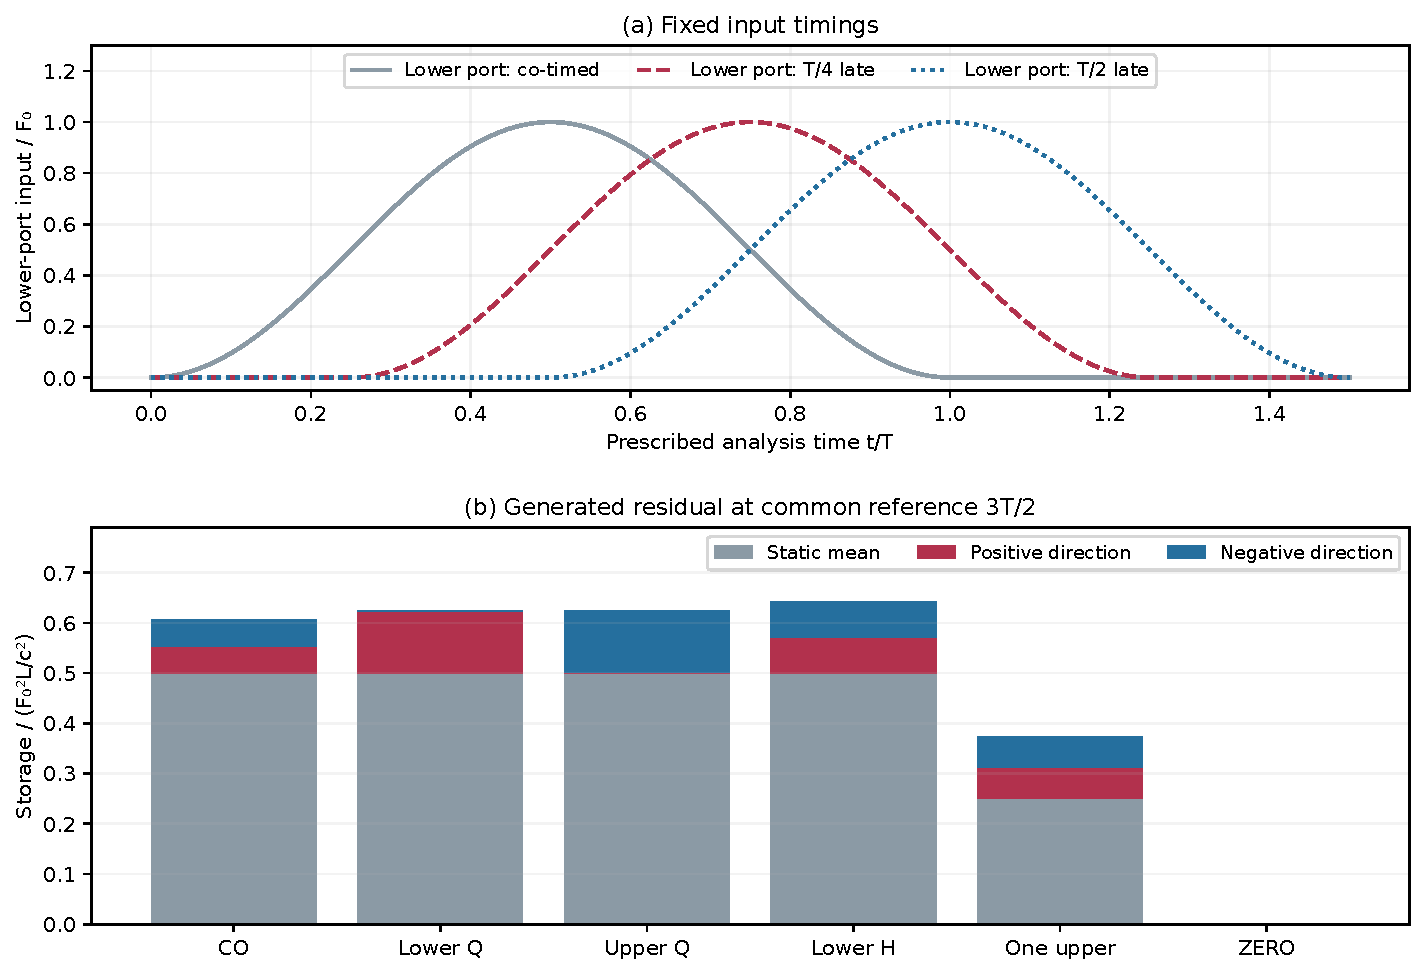
\includegraphics[width=\textwidth]{figures/timing.pdf}
\caption{Fixed prescribed delays and generated directional account, using the retained SRG-08 schedule and storage data. Every control uses the common $3T/2$ reference; no per-control rephasing or amplitude normalization is used. The weak direction of the quarter controls remains nonzero. The mean is the largest storage component.}\label{fig:timing}
\end{figure}

\subsection{Swapped timing in the actual exterior records}\label{sec:swap}
For all timing controls use the common late window
\begin{equation}\label{eq:timingwindow}
 [\tref+D_{\max}/c_e,\tref+D_{\max}/c_e+T],\qquad \tref=3T/2.
\end{equation}
Every delayed argument is at least $3T/2$, hence after the latest switch-off. In units $g_oF_0/c$, the record is
\begin{equation}\label{eq:timingrecord}
 (D_X\bar p c/F_0,0,0,0)\tr+
 \Re\left\{Q_X(\nu)\frac c{F_0}\binom{a_+}{a_-}
 e^{\ii\omega(t-3T/2)}\right\}.
\end{equation}
The amplitudes are the newly generated ones in \eqref{eq:lagamp}, not the common-envelope matrix $N$ applied outside its domain. Earlier records use the actual finite histories in \eqref{eq:composition}.

\begin{proposition}[Swapped-input distinction and its nulls]\label{prop:swap}
Equatorial scalar records of the two quarter-delay controls are identical throughout their causal histories, at every exterior speed. At $\nu=0,1$, their known-clock late scalar records differ at each retained off-height site, and their full records differ at every retained site. Scalar and total period mean-square records remain identical everywhere.
\end{proposition}
\begin{proof}
Reflection and uniqueness give $p_{\rm exchanged}(s,t)=p(L-s,t)$ and $r_{\rm exchanged}(s,t)=-r(L-s,t)$. At equatorial sites $d(s)=d(L-s)$, so reflected scalar contributions have identical delay and integrate to the same causal record. This is stronger than a late phasor collision.

Write $A=a_+$, $B=a_-$ for lower-late Q. Upper-late exchanges them. The scalar late difference is
$-2\ii g_oH(A-B)\sin\phi$. At off-height sites $\sin\phi\ne0$, $H\ne0$ by the sector theorem, and $A-B\ne0$ by \eqref{eq:quarter}, so it is nonzero. Full $Q_X$ has rank two and therefore distinguishes any distinct amplitude pairs.

For the squared records, $A,B$ have one common complex phase times real coefficients. Thus $A\overline B$ is real and unchanged by exchange. For any row $q=(q_+,q_-)$, expansion yields
\begin{equation}\label{eq:swap_power}
 |q_+A+q_-B|^2-|q_+B+q_-A|^2
 =(|A|^2-|B|^2)(|q_+|^2-|q_-|^2).
\end{equation}
The scalar column magnitudes are equal, as are the full column norms by \eqref{eq:reduction}. Their squared differences are therefore zero. The two controls have the same DC, whose cross term with a harmonic averages to zero over a period. Hence their scalar and total mean squares coincide as claimed.
\end{proof}

Individual vector components have column-square difference
$-4\Im(S_m\overline{C_m})(B\tr e_q)_j(B\tr e_\perp)_j$. It vanishes for real moments at $\nu=0$, and at equatorial sites in the fixed frames for any delay. The retained $\nu=1$ data distinguish at least one component at every fixed off-height site, with margins above their allowances. This is a finite fixture finding, not an all-position theorem or a received-energy law.

A single off-height scalar phasor distinguishes two known hypotheses but cannot invert two arbitrary complex amplitudes. With an unknown scalar clock phase, the two quarter records at one site can be made identical because they have equal magnitude and DC. A known common phase across an independent scalar stack permits a ratio inverse; independent site clocks defeat that argument. Full within-site channels retain the amplitude ratio if their nuisance factor is common. That ratio determines $\eta_{\rm osc}$, but $\eta_{\rm total}$ also needs the mean/harmonic relative calibration. A common absolute gain cancels from that relative account only if it applies to both DC and harmonic records.

For inherited matrix error $e_Q$, the phasor allowance propagates as $e_Q\norm{(a_+,a_-)}$ plus output rounding. The source record uses the old analytic truncation bound, $\sqrt8\,10^{-14}$ serialized matrix allowance, $10^{-45}$ arithmetic allowance and $10^{-14}$ output allowance. Differences add their individual bounds; stacks combine in quadrature; summaries carry $10^{-11}$. For squared magnitudes, $||z+\delta z|^2-|z|^2|\le2|z||\delta z|+|\delta z|^2$ propagates those allowances, with the period factor $1/2$. None is a formally directed-rounded enclosure. The exact scalar null and rank theorems do not rest on the numerical tables.
